\documentclass[aspectratio=169,10pt]{beamer}

\usepackage[T1]{fontenc}
\usepackage[utf8]{inputenc}
\usepackage[scaled=0.95]{helvet}
\usepackage{lmodern}
\usepackage{microtype}
\usepackage{graphicx}
\usepackage{booktabs}
\usepackage{tabularx}
\usepackage{array}
\usepackage{amsmath, amssymb}
\usepackage{siunitx}
\usepackage{tikz}
\usetikzlibrary{arrows.meta, positioning, fit, calc}

\graphicspath{{figures/}{presentation_figures/}{../experiments/plots/}}
\setbeamertemplate{navigation symbols}{}
\setbeamersize{text margin left=0.75cm, text margin right=0.75cm}
\setlength{\tabcolsep}{6pt}
\renewcommand{\familydefault}{\sfdefault}

\definecolor{Ink}{HTML}{1D2E36}
\definecolor{Stone}{HTML}{65737E}
\definecolor{Sand}{HTML}{F5F1EA}
\definecolor{Teal}{HTML}{0F6D74}
\definecolor{Orange}{HTML}{D97706}
\definecolor{Sky}{HTML}{E9F4F4}

\setbeamercolor{normal text}{fg=Ink,bg=white}
\setbeamercolor{frametitle}{fg=Ink,bg=white}
\setbeamercolor{title}{fg=Ink}
\setbeamercolor{subtitle}{fg=Stone}
\setbeamercolor{block title}{fg=white,bg=Teal}
\setbeamercolor{block body}{fg=Ink,bg=Sand}
\setbeamercolor{block title alerted}{fg=white,bg=Orange}
\setbeamercolor{block body alerted}{fg=Ink,bg=Orange!10}
\setbeamercolor{block title example}{fg=white,bg=Ink}
\setbeamercolor{block body example}{fg=Ink,bg=Sky}
\setbeamertemplate{blocks}[rounded][shadow=false]
\setbeamerfont{title}{size=\fontsize{22}{26}\selectfont,series=\bfseries}
\setbeamerfont{frametitle}{size=\Large,series=\bfseries}
\setbeamerfont{block title}{series=\bfseries}

\setbeamertemplate{frametitle}{
  \vspace{0.15cm}
  \begin{beamercolorbox}[wd=\paperwidth,ht=0.95cm,dp=0.18cm,leftskip=0.75cm,rightskip=0.75cm]{frametitle}
    \usebeamerfont{frametitle}\insertframetitle
  \end{beamercolorbox}
}

\setbeamertemplate{footline}{
  \leavevmode
  \begin{beamercolorbox}[wd=\paperwidth,ht=0.34cm,dp=0.14cm]{author in head/foot}
    \hspace*{0.75cm}\color{Stone}\scriptsize CS566 Term Project Presentation
    \hfill
    \color{Stone}\scriptsize \insertframenumber/\inserttotalframenumber\hspace*{0.75cm}
  \end{beamercolorbox}
}

\newcommand{\pill}[1]{%
  \tikz[baseline=(node.base)]\node[
    rounded corners=8pt,
    fill=Sky,
    draw=Teal!35,
    inner xsep=7pt,
    inner ysep=3pt
  ] (node) {\scriptsize #1};%
}

\title{Attention-Augmented Scale Hyperprior\\for Learned Image Compression}
\subtitle{CS566 Deep Learning Term Project}
\author{Emre Y{\i}lmaz}
\date{Spring 2026}

\begin{document}

\begin{frame}[plain]
  \begin{tikzpicture}[remember picture, overlay]
    \fill[Sand] (current page.south west) rectangle ([xshift=4.1cm]current page.north west);
    \fill[Orange] (current page.south west) rectangle ([xshift=0.20cm]current page.north west);
    \fill[Teal!10] ([xshift=-0.8cm,yshift=-0.9cm]current page.north east) circle (1.9cm);
    \fill[Orange!12] ([xshift=-1.2cm,yshift=0.8cm]current page.south east) circle (1.4cm);
  \end{tikzpicture}

  \vspace*{0.55cm}
  {\large\color{Stone}CS566 Deep Learning Term Project\par}
  \vspace{0.35cm}
  {\usebeamerfont{title}\color{Ink}\inserttitle\par}
  \vspace{0.45cm}
  {\large\color{Stone}\insertauthor\par}
  {\normalsize\color{Stone}\insertdate\par}

  \vspace{0.65cm}
  \begin{beamercolorbox}[wd=0.72\paperwidth,rounded=true,sep=0.9em,leftskip=0.25cm]{block body alerted}
    \large \textbf{Main takeaway:} the SE blocks were easy to integrate and lightweight,
    but they did not produce a meaningful Kodak rate-distortion gain.
  \end{beamercolorbox}
\end{frame}

\begin{frame}{Problem \& Motivation}
  \begin{columns}[T,onlytextwidth]
    \column{0.32\textwidth}
    \begin{block}{Problem}
      Images need to be compressed to a low bitrate \emph{without} visibly damaging reconstruction quality.
    \end{block}

    \column{0.32\textwidth}
    \begin{block}{Why Learned Compression}
      Neural codecs can learn the encoder, latent prior, and decoder jointly for rate-distortion optimization.
    \end{block}

    \column{0.32\textwidth}
    \begin{alertblock}{Project Objective}
      Keep the Ball\'e scale hyperprior fixed and test whether lightweight SE attention improves compression.
    \end{alertblock}
  \end{columns}

  \vspace{0.4cm}
  \begin{exampleblock}{Fair Experimental Question}
    Compare a fine-tuned vanilla baseline (\(A_{\mathrm{ft}}\)) against two SE variants:
    encoder-only (\(B\)) and encoder+decoder (\(C\)), using \textbf{true coded bitrate} on Kodak.
  \end{exampleblock}
\end{frame}

\begin{frame}{Dataset \& Experimental Setup}
  \begin{columns}[T,onlytextwidth]
    \column{0.40\textwidth}
    \begin{block}{Final Setup}
      \begin{itemize}
        \item CLIC train/val: 1,633 / 102
        \item Kodak test: 24 images
        \item \(256\times256\) crops; 4 \(\lambda\) values
      \end{itemize}
    \end{block}

    \column{0.56\textwidth}
    \begin{center}
      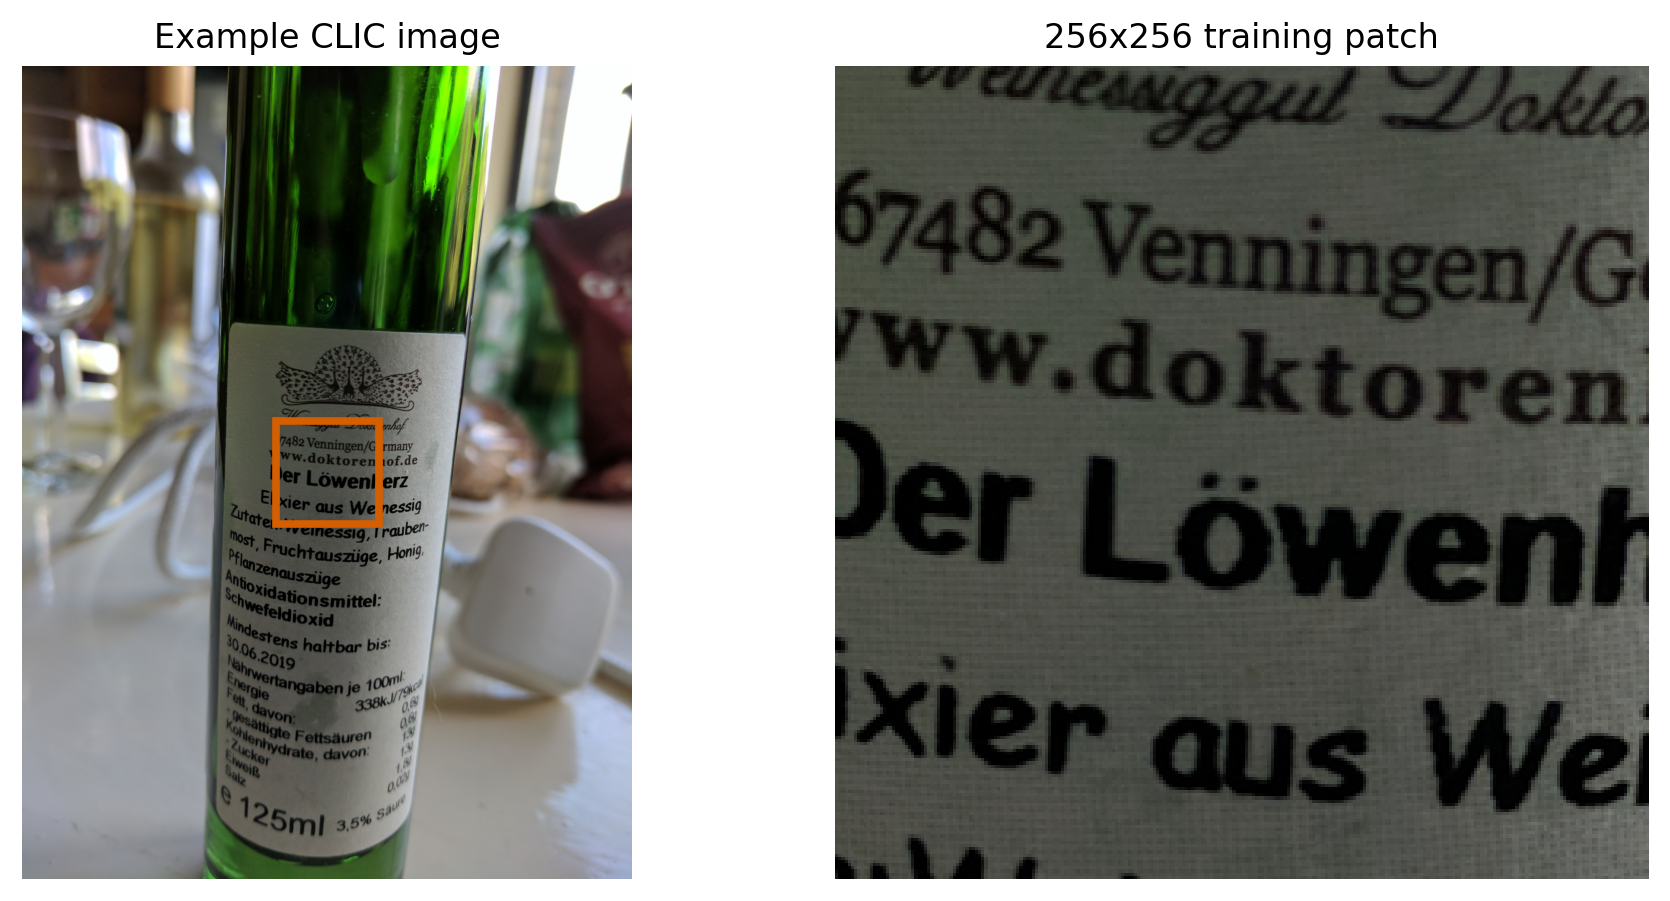
\includegraphics[width=0.98\linewidth]{preprocessing_patch_example.png}
    \end{center}
  \end{columns}
\end{frame}

\begin{frame}{Method Overview}
  \begin{center}
    \resizebox{0.98\linewidth}{!}{%
      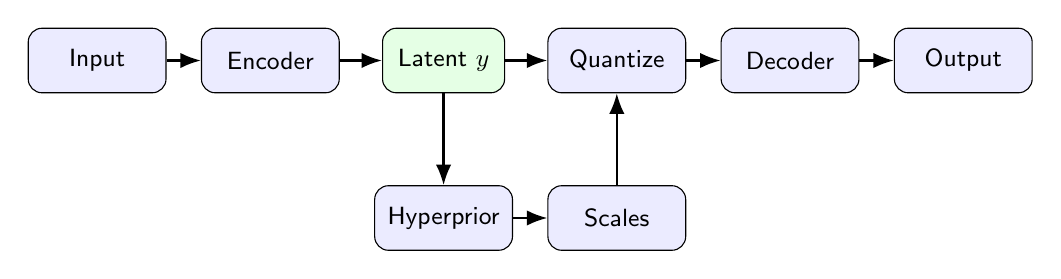
\begin{tikzpicture}[
        font=\small,
        overviewbox/.style={draw, rounded corners=5pt, minimum width=1.75cm, minimum height=0.82cm, align=center, fill=blue!8},
        latentbox/.style={draw, rounded corners=5pt, minimum width=1.55cm, minimum height=0.82cm, align=center, fill=green!10},
        arr/.style={-{Latex[length=2.6mm]}, thick, color=black}
      ]
        \node[overviewbox] (input) at (0.0,0.0) {Input};
        \node[overviewbox] (enc) at (2.2,0.0) {Encoder};
        \node[latentbox] (latent) at (4.4,0.0) {Latent \(y\)};
        \node[overviewbox] (quant) at (6.6,0.0) {Quantize};
        \node[overviewbox] (dec) at (8.8,0.0) {Decoder};
        \node[overviewbox] (out) at (11.0,0.0) {Output};

        \node[overviewbox] (hyper) at (4.4,-2.0) {Hyperprior};
        \node[overviewbox] (scales) at (6.6,-2.0) {Scales};

        \draw[arr] (input) -- (enc);
        \draw[arr] (enc) -- (latent);
        \draw[arr] (latent) -- (quant);
        \draw[arr] (quant) -- (dec);
        \draw[arr] (dec) -- (out);

        \draw[arr] (latent) -- (hyper);
        \draw[arr] (hyper) -- (scales);
        \draw[arr] (scales) -- (quant);
      \end{tikzpicture}%
    }
  \end{center}

  \vspace{0.25cm}
  \begin{exampleblock}{What Changes and What Stays Fixed}
    \textbf{Changed:} SE blocks are added in the transform network (encoder in \(B\), encoder+decoder in \(C\)).\\[0.08cm]
    \textbf{Fixed:} the hyperprior, scale prediction, quantization, and entropy model stay the same.
  \end{exampleblock}
\end{frame}

\begin{frame}{Model Architecture}
  \begin{columns}[T,onlytextwidth]
    \column{0.60\textwidth}
    \begin{center}
      \resizebox{\linewidth}{!}{%
        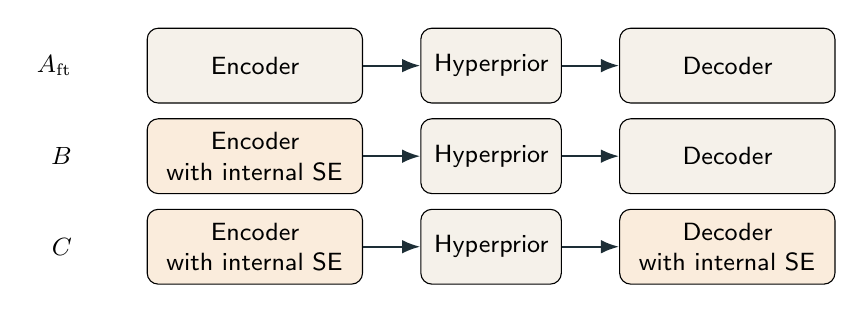
\begin{tikzpicture}[
          font=\small,
          row/.style={draw, rounded corners=4pt, minimum height=0.95cm, align=center, fill=Sand},
          transform/.style={row, text width=2.5cm},
          priorblock/.style={row, text width=1.55cm},
          highlighted/.style={row, text width=2.5cm, fill=Orange!14},
          arr/.style={-{Latex[length=2.3mm]}, thick, color=Ink}
        ]
          \node[anchor=east] at (0.8,1.15) {\(A_{\mathrm{ft}}\)};
          \node[transform] (a1) at (3.0,1.15) {Encoder};
          \node[priorblock] (a2) at (6.0,1.15) {Hyperprior};
          \node[transform] (a3) at (9.0,1.15) {Decoder};
          \draw[arr] (a1) -- (a2);
          \draw[arr] (a2) -- (a3);

          \node[anchor=east] at (0.8,0) {\(B\)};
          \node[highlighted] (b1) at (3.0,0) {Encoder\\with internal SE};
          \node[priorblock] (b2) at (6.0,0) {Hyperprior};
          \node[transform] (b3) at (9.0,0) {Decoder};
          \draw[arr] (b1) -- (b2);
          \draw[arr] (b2) -- (b3);

          \node[anchor=east] at (0.8,-1.15) {\(C\)};
          \node[highlighted] (c1) at (3.0,-1.15) {Encoder\\with internal SE};
          \node[priorblock] (c2) at (6.0,-1.15) {Hyperprior};
          \node[highlighted] (c3) at (9.0,-1.15) {Decoder\\with internal SE};
          \draw[arr] (c1) -- (c2);
          \draw[arr] (c2) -- (c3);
        \end{tikzpicture}%
      }
    \end{center}

    \column{0.36\textwidth}
    \begin{block}{Implemented Details}
      \small
      \begin{itemize}
        \item \(B\): SE after encoder conv 2
        \item \(C\): + decoder SE after deconv 2
        \item Pretrained transfer; \(+2.2\text{k} / +4.4\text{k}\) params
      \end{itemize}
    \end{block}
  \end{columns}
\end{frame}

\begin{frame}{SE Block: General Idea}
  \begin{center}
    \resizebox{0.92\linewidth}{!}{%
      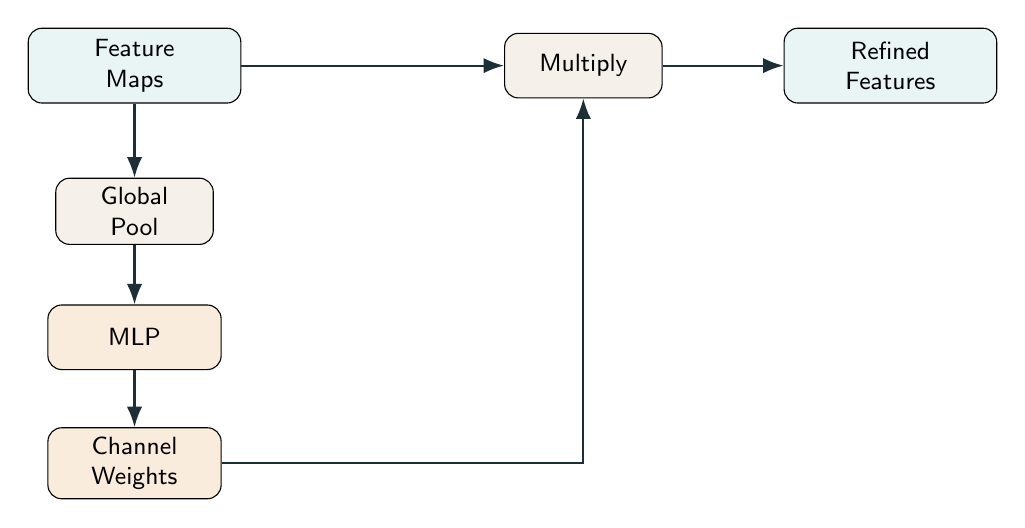
\begin{tikzpicture}[
        font=\small,
        feature/.style={draw, rounded corners=5pt, minimum width=2.7cm, minimum height=0.95cm, align=center, fill=Sky},
        op/.style={draw, rounded corners=5pt, minimum width=2.0cm, minimum height=0.82cm, align=center, fill=Sand},
        gate/.style={draw, rounded corners=5pt, minimum width=2.2cm, minimum height=0.82cm, align=center, fill=Orange!14},
        arr/.style={-{Latex[length=2.6mm]}, thick, color=Ink}
      ]
        \node[feature] (x) at (0.0,0.0) {Feature\\Maps};
        \node[op] (mul) at (5.7,0.0) {Multiply};
        \node[feature] (out) at (9.6,0.0) {Refined\\Features};

        \node[op] (pool) at (0.0,-1.85) {Global\\Pool};
        \node[gate] (mlp) at (0.0,-3.45) {MLP};
        \node[gate] (weights) at (0.0,-5.05) {Channel\\Weights};

        \draw[arr] (x.east) -- (mul.west);
        \draw[arr] (mul.east) -- (out.west);

        \draw[arr] (x.south) -- (pool.north);
        \draw[arr] (pool.south) -- (mlp.north);
        \draw[arr] (mlp.south) -- (weights.north);
        \draw[arr] (weights.east) -| (mul.south);
      \end{tikzpicture}%
    }
  \end{center}
\end{frame}

\begin{frame}{Training Objective}
  \begin{alertblock}{Rate-Distortion Loss}
    \[
      \mathcal{L} = \lambda D(x,\hat{x}) + R(\hat{y}) + R(\hat{z})
    \]
  \end{alertblock}

  \begin{columns}[T,onlytextwidth]
    \column{0.48\textwidth}
    \begin{block}{Training Setup}
      \centering
      4 operating points\\[0.18cm]
      Adam: \(10^{-4}\) backbone, \(10^{-3}\) SE
    \end{block}

    \column{0.48\textwidth}
    \begin{exampleblock}{Evaluation}
      \centering
      PSNR\\[0.18cm]
      true coded bitrate
    \end{exampleblock}
  \end{columns}
\end{frame}

\begin{frame}{Results: RD Curves}
  \begin{columns}[T,onlytextwidth]
    \column{0.48\textwidth}
    
\includegraphics[width=\linewidth,height=0.56\textheight,keepaspectratio]{rd_curve_psnr_project_zoom.pdf}

    \column{0.48\textwidth}
    
\includegraphics[width=\linewidth,height=0.56\textheight,keepaspectratio]{rd_curve_msssim_project_zoom.pdf}
  \end{columns}

  \vspace{0.05cm}
  \begin{exampleblock}{Takeaway}
    \centering
    \large project curves nearly overlap
  \end{exampleblock}
\end{frame}

\begin{frame}{Results: BD-Rate Summary}
  \begin{columns}[T,onlytextwidth]
    \column{0.68\textwidth}
    
\includegraphics[width=\linewidth,height=0.62\textheight,keepaspectratio]{bd_rate_psnr.pdf}

    \column{0.28\textwidth}
    \begin{alertblock}{Takeaway}
      \small
      \begin{itemize}
        \setlength{\itemsep}{0.18em}
        \item \(B\): \(+0.08\%\)
        \item \(C\): \(+0.17\%\)
        \item Stronger priors: \(-8\%\) to \(-25\%\)
      \end{itemize}
    \end{alertblock}
  \end{columns}
\end{frame}

\begin{frame}{Runtime Evaluation}
  \begin{columns}[T,onlytextwidth]
    \column{0.52\textwidth}
    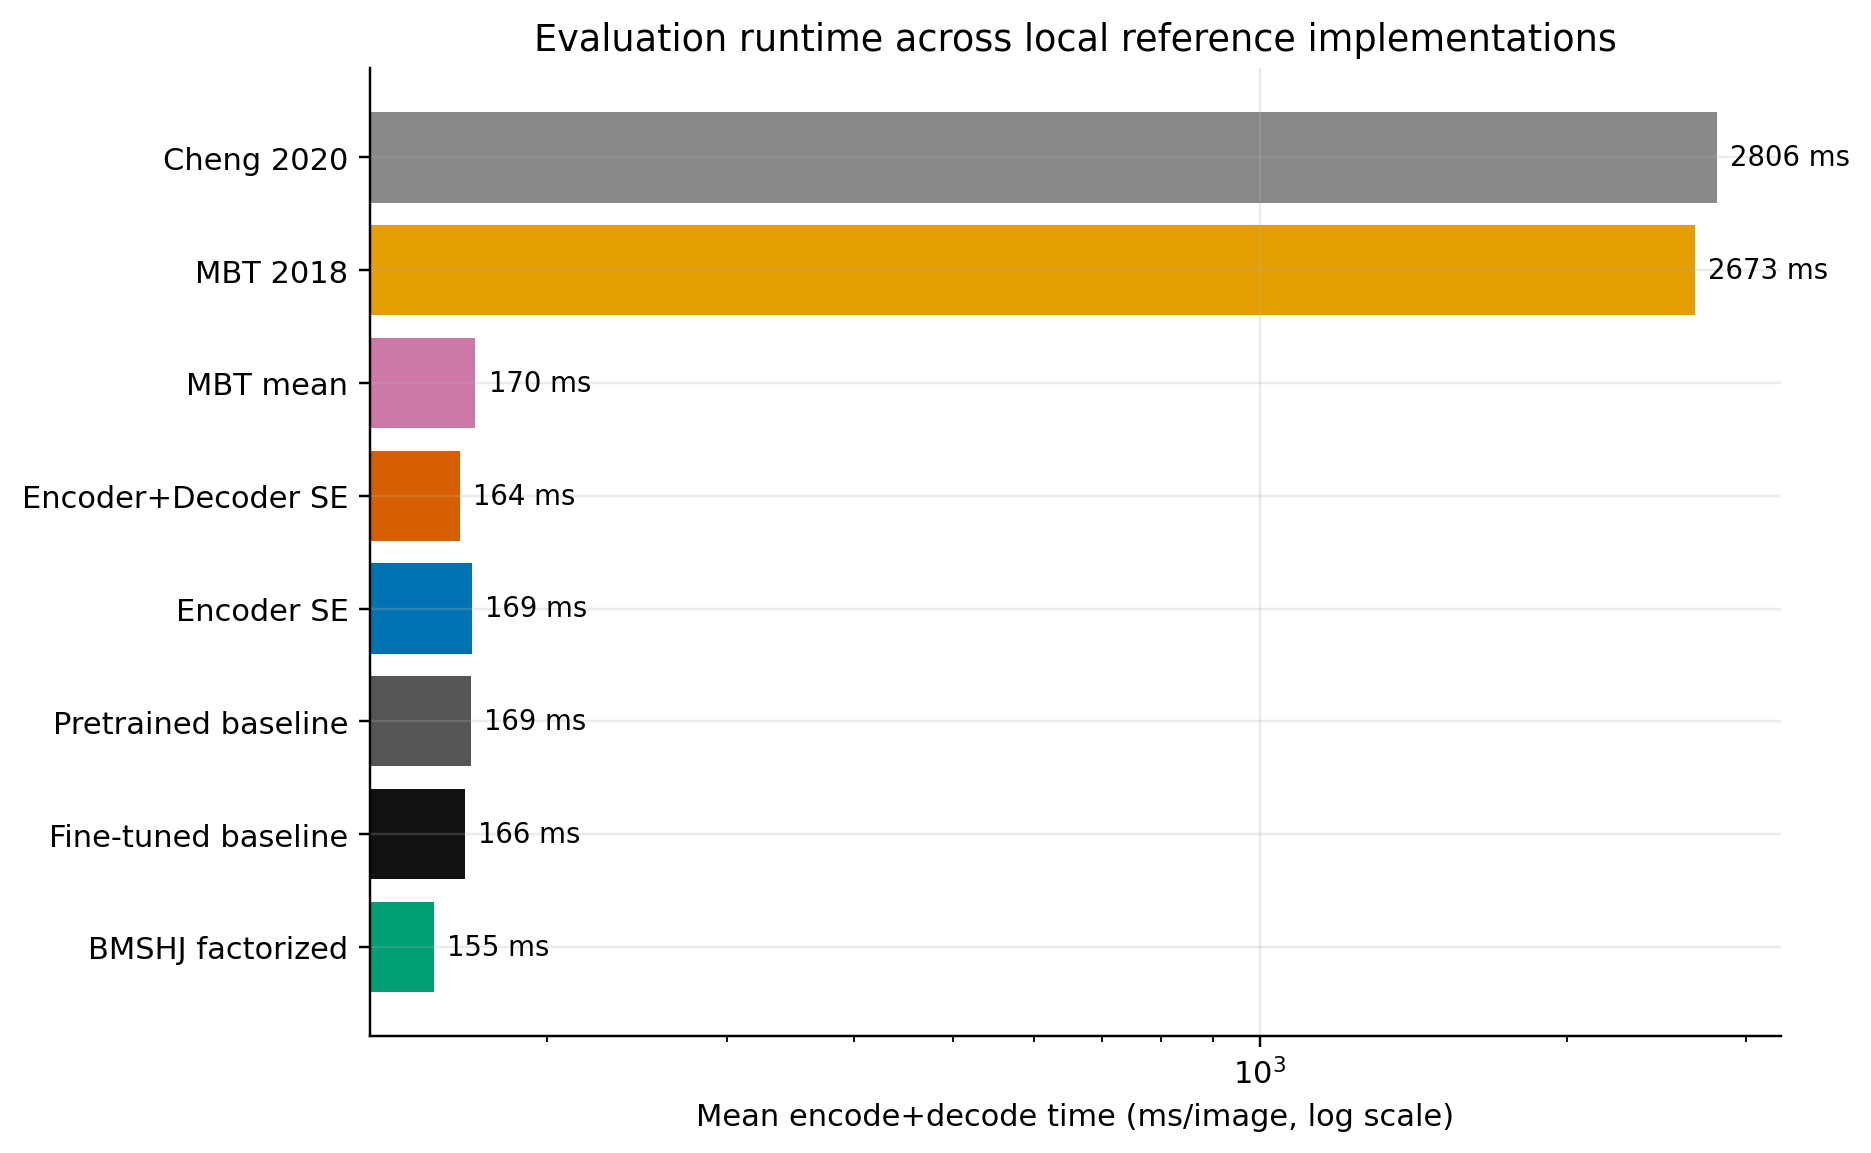
\includegraphics[width=\linewidth]{runtime_comparison_all.png}

    \column{0.44\textwidth}
    \begin{block}{Runtime and Params}
      \centering
      \scriptsize
      \begin{tabular}{lccc}
        \toprule
        Variant & Params & Fwd & Codec \\
         & (M) & (ms) & (ms) \\
        \midrule
        \(A_{\mathrm{ft}}\) & 5.1 & 11.4 & 166 \\
        \(B\) & 5.1 & 11.6 & 169 \\
        \(C\) & 5.1 & 11.7 & 164 \\
        BMSHJ & 3.0 & 10.4 & 155 \\
        MBT mean & 7.0 & 11.4 & 170 \\
        MBT & 14.1 & 16.0 & 2673 \\
        Cheng & 11.833 / 26.599* & 26.2 & 2806 \\
        \bottomrule
      \end{tabular}

      \vspace{0.08cm}

      {\tiny\color{Stone}\raggedright
      * Cheng 2020 anchor uses 11.833M parameters for qualities 1--3 and 26.599M for quality 4.\par}
    \end{block}
  \end{columns}
\end{frame}

\begin{frame}{Image Comparison}
  \begin{center}
    \begin{columns}[T,onlytextwidth]
      \column{0.24\textwidth}
      {\scriptsize\centering Input\par}
      \column{0.24\textwidth}
      {\scriptsize\centering Baseline FT\par}
      \column{0.24\textwidth}
      {\scriptsize\centering Encoder SE\par}
      \column{0.24\textwidth}
      {\scriptsize\centering Encoder+Decoder SE\par}
    \end{columns}

    \vspace{0.08cm}
    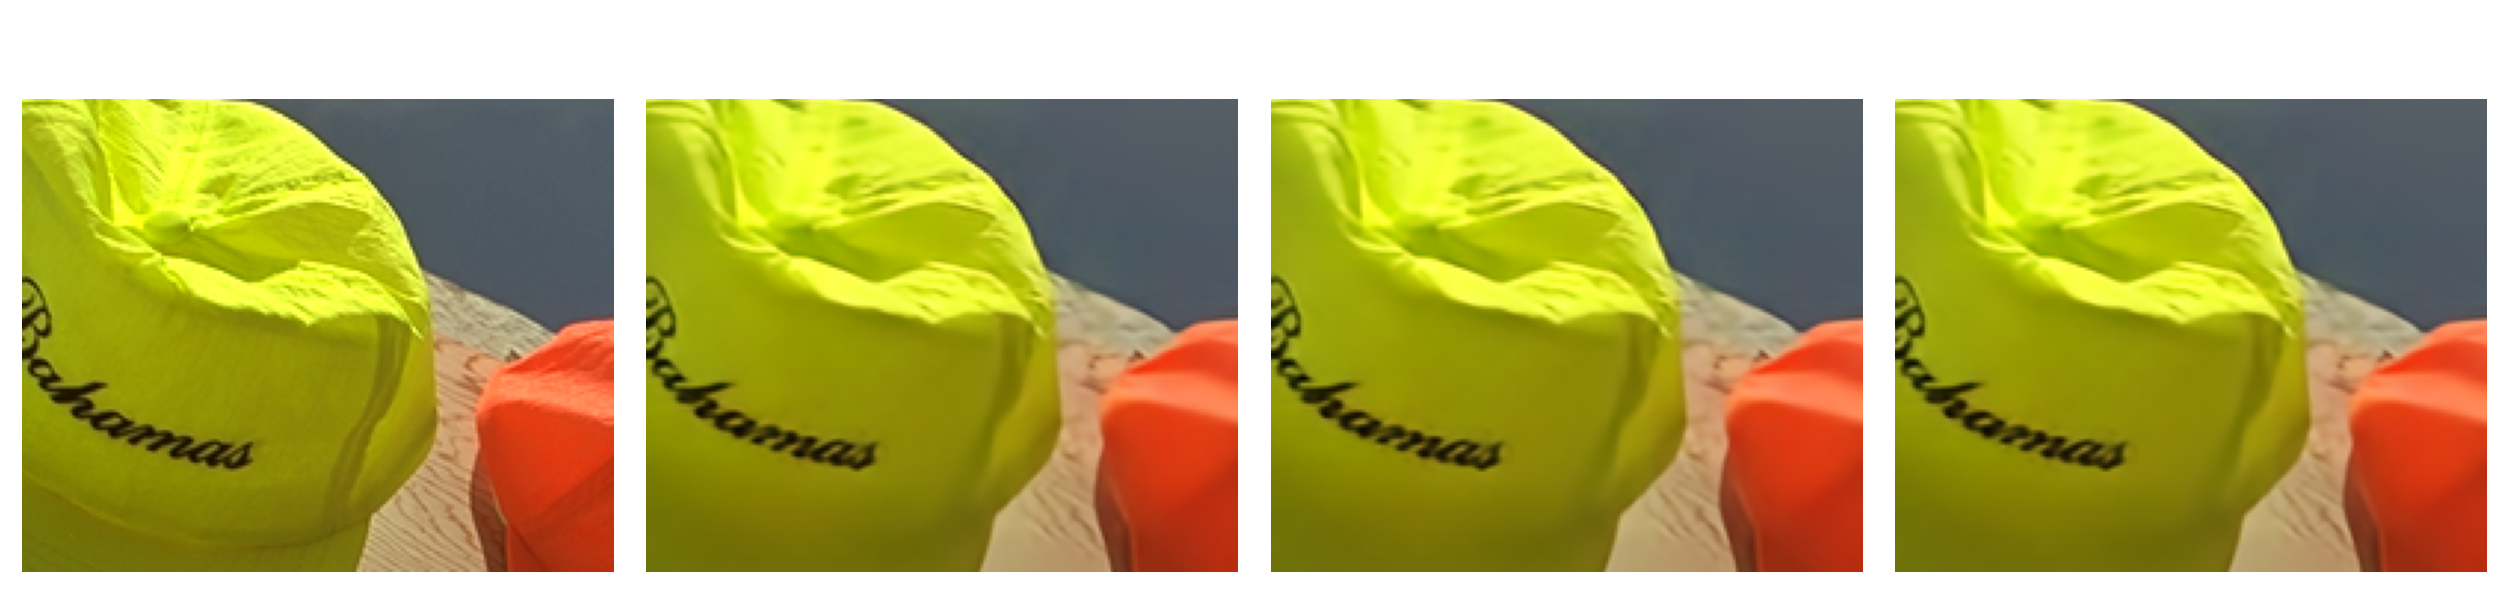
\includegraphics[width=0.92\linewidth]{reconstruction_panel_q3_kodim03_zoom_only.png}

    \vspace{0.14cm}
    {\small\color{Stone}\centering no visible difference at quality level 3\par}
  \end{center}
\end{frame}

\begin{frame}{Discussion}
  \begin{alertblock}{Why SE Did Not Help Much Here}
    \small
    \begin{itemize}
      \item \textbf{No visual gain:} all variants look the same at quality level 3.
      \item \textbf{Global blanket:} one weight scales an entire channel everywhere.
      \item \textbf{Background bottleneck:} flat regions get boosted along with useful detail, wasting bits.
      \item \textbf{Why Cheng 2020 helps:} spatial attention can suppress flat areas and preserve details.
    \end{itemize}
  \end{alertblock}
\end{frame}

\begin{frame}{Conclusion}
  \begin{columns}[T,onlytextwidth]
    \column{0.32\textwidth}
    \begin{block}{1. Implemented}
      Two SE-augmented scale-hyperprior variants, pretrained weight transfer, fair baselines, ablations, and cleaned evaluation.
    \end{block}

    \column{0.32\textwidth}
    \begin{alertblock}{2. Main Result}
      On Kodak, the SE variants do \textbf{not} show a meaningful rate-distortion gain over the fine-tuned vanilla baseline.
    \end{alertblock}

    \column{0.32\textwidth}
    \begin{block}{3. Takeaway}
      Lightweight transform-side attention is easy to add, but stronger priors and context models are the more promising direction.
    \end{block}
  \end{columns}
\end{frame}

\begin{frame}[plain]
  \begin{center}
    \vspace{1.8cm}
    {\usebeamerfont{title}\color{Ink}Thank you\par}
    \vspace{0.45cm}
    {\Large\color{Stone}Questions?\par}
  \end{center}
\end{frame}

\end{document}
